%\section{Grundlagen}

\section{Aufbau}
Ein neuronales Netz besteht aus mehreren Neuronen, die miteinander verbunden sind. Ein Neuron kann wie in Abbildung \ref{neuron} modelliert werden. Demzufolge besteht ein Neuron aus einer Menge an Inputs und einem Output. Die gewichteten Inputs werden kumuliert und in eine Aktivierungsfunktion eingesetzt. Dieses Ergebnis geht dann als Output an weitere Neuronen. 
\begin{figure}[h]
\centering
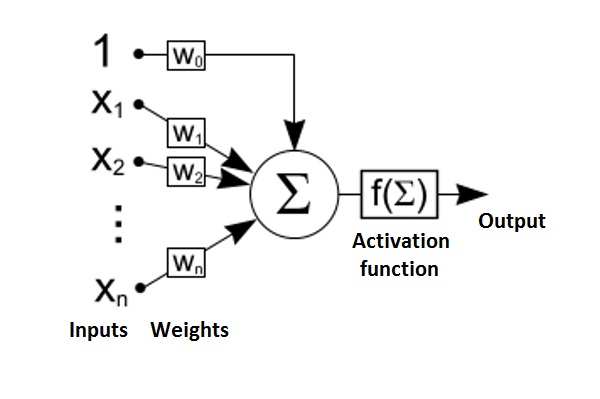
\includegraphics[width=0.6\textwidth]{pictures/neuron.jpg}
\caption{Modell eines Neurons \cite{bib:neuron}}
\label{neuron}
\end{figure}

Durch das Verbinden der einzelnen Neuronen ergibt sich ein Netz. Dieses wird in Schichten unterteilt, damit es übersichtlicher und beherrschbarer wird. Abbildung \ref{network} zeigt ein solches Modell.
\begin{figure}[h]
\centering
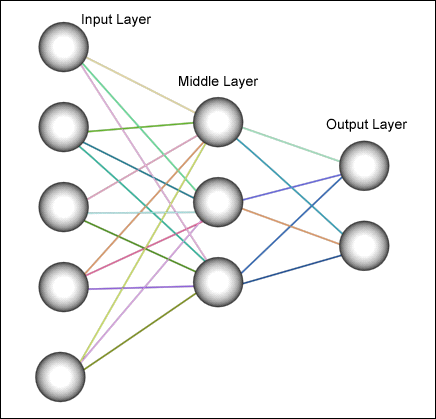
\includegraphics[width=0.5\textwidth]{pictures/neural-network.png}
\caption{Modell eines neuronalen Netzes \cite{bib:neuron}}
\label{network}
\end{figure}

Das dargestellte Modell besteht aus einem Input-Layer, der nur als Interface zwischen dem Netz und seiner Umgebung dient, einem Middel Layer, auch Hidden-Layer genannt, sowie einem Output-Layer, das die Systemantwort des Netzes an die Umgebung ausgibt. Der Name \emph{Hidden-Layer} bezieht sich darauf, dass diese Zwischenschicht von außen nicht einsehbar ist.

Damit das Modell eines neuronalen Netzes arbeiten kann, ist es notwendig, die einzelnen Vorgänge mathematisch darzustellen. Diese mathematischen Eigenschaften eines neuronalen Netzes sollen im Folgenden beschrieben werden. Die verwendeten Formeln entstammen dem Skript der Vorlesung \emph{Digitale Sprachverarbeitung} 2011 von Dr. Thomas Dörsam.

\section{Eingang}
Ein Neuron reagiert auf Eingänge, wenn sie bestimmte Bedingungen erfüllen. Der Wert, der von außen auf das Neuron wirkt, wird \emph{Eingangserregung} genannt. Die Bedingungen, die erfüllt sein müssen, werden \emph{Aktivierungsfunktion} genannt.

\subsection{Eingangserregung}
Damit ein Neuron des Netzes überhaupt reagieren kann, ist es notwendig, alle eingehenden Werte unter Berücksichtigung ihrer Gewichte miteinander zu kumulieren. Dies geschieht über eine Erregungsfunktion. Es gibt keine Vorschriften für eine solche Erregungsfunktion. Typisch sind jedoch das Skalarprodukt, oder die euklidische Distanz. Diese Erregungsfunktionen $\sigma$ für ein j-tes Neurons mit n Eingängen lauten:

Skalarprodukt:
\begin{equation}
  \sigma_{j} = \sum_{i=1}^{n} w_{ji} x_{i}+w_{j0}
\end{equation} 

Euklidische Distanz:
\begin{equation}
  \sigma_{j} = \sum_{i=1}^{n} (w_{ji} - x_{i})^2+w_{j0}^2
\end{equation} 

\subsection{Aktivierungsfunktion}
Nachdem der kumulierte Erregungswert $\sigma$ mit Hilfe einer Erregungsfunktion berechnet wurde, muss ermittelt werden, wie stark dieser Wert das Neuron aktiviert. Hierfür stehen ebenfalls diverse Funktionen zu Auswahl.

Eine klassische Schwellwertfunktion ist die Stufenfunktion. Wird ein bestimmter Wert überschritten, wird das Neuron aktiviert und beginnt zu feuern (Abbildung \ref{stufe}).
\begin{equation}
f(\sigma) = 1 \mbox{ if } \sigma < 0;  \mbox{ else } 0
\end{equation}
\begin{figure}[h]
\centering
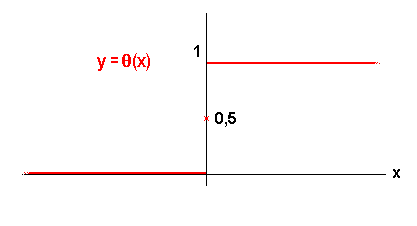
\includegraphics[width=0.6\textwidth]{pictures/stufenfunktion.png}
\caption{Stufenfunktion \cite{bib:stufe}}
\label{stufe}
\end{figure}

Da die Stufenfunktion das Verhalten eines Neurons sehr gut abbildet, allerdings nicht stetig und damit nicht vollständig differenzierbar ist, wird sie durch die Sigmoidfunktion (Abbildung \ref{sigmoid}) angenähert. Diese erhält den Schwellwertcharakter der Stufenfunktion, steigt aber flacher an und umgeht so die Unstetigkeit.
\begin{equation}
f(\sigma) = \frac{1}{1+e^{-\sigma}}
\end{equation}
\begin{figure}[h]
\centering
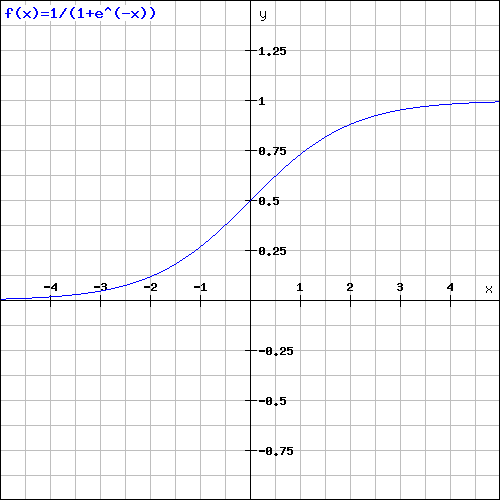
\includegraphics[width=0.6\textwidth]{pictures/sigmoid.png}
\caption{Sigmoidfunktion}
\label{sigmoid}

\end{figure}

Ein weiterer Vorteil der Sigmoidfunktion ist die sehr einfache Ableitung, die eine effiziente Implementierung ermöglicht.
\begin{equation}
f'(\sigma) = f(\sigma)\cdot (1- f(\sigma))
\end{equation}

Soll das Neuron nur innerhalb eines bestimmten Bereichs aktiviert werden, eignet sich eine Glockenfunktion (Abbildung  \ref{glocke}). Sie approximiert eine Fensterfunktion, ist aber ebenfalls stetig.
\begin{equation}
f(\sigma) = e^{-\sigma^2}
\end{equation}
\begin{figure}[h]
\centering
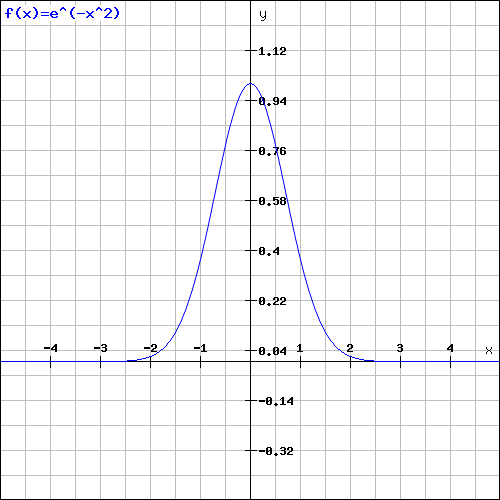
\includegraphics[width=0.6\textwidth]{pictures/glocke.png}
\caption{Glockenfunktion}
\label{glocke}
\end{figure}

\section{Feedforward Berechnung}
Nachdem nun die Eigenschaften eines einzelnen Neurons definiert wurden, ist es möglich den gesamten Output eines ganzen Netzes zu berechnen.  Es wird jeweils der Input der vorherigen Schicht kumuliert und das Ergebnis der Aktivierungsfunktion an die nachfolgende Schicht weitergegeben. Für die nachfolgende Formel wurde das Skalarprodukt, sowie ein Hidden-Layer zugrunde gelegt. Bei mehr Hidden-Layern müsste die Funktion diese ebenso als Summe verschachteln.
\begin{equation}
o_{k}(\vec{x})=f\left( \sum_{j=1}^{n_{hidden}} w_{kj} f\left(\sum_{i=1}^{n_{input}} w_{ji}x_{i}+w_{j0} \right)+w_{k0} \right)
\label{eq:o}
\end{equation}
Um die vollständige Systemantwort zu erhalten, muss diese Funktion für jedes Neuron des Output-Layers berechnet werden.

\section{Training}

Damit ein neuronales Netz eine adäquate Systemantwort generieren kann, ist es not\-wen\-dig das Netz zu trainieren. In der Natur geschieht dies, indem die einzelnen Verbindungen zwischen zwei Neuronen dicker werden, oder sogar neue entstehen. Zumindest das Wachstum der Verbindungen lässt sich im mathematischen Modell durch die Modifikation der Gewichte nachbilden. Wichtige Neuronen werden ungefiltert, oder sogar verstärkt in den Erregungswert einfließen, unwichtige, oder sogar störende Neuronen werden gedämpft.

Um das neuronale Netz zu trainieren muss ein Teil der zu analysierenden Daten manuell bearbeitet werden. Die eine Hälfte dieses Datensatzes wird zum Training des Netzes eingesetzt, der Andere zur Verifikation der Arbeitsweise.
 
Beim Training des Netzes wird die generierte Systemantwort o des Output-Neurons k mit dem gewünschten Ergebnis t verglichen und die Differenz $t_k - o_k$ berechnet. Da nur der absolute Abstand wichtig ist, müsste eigentlich der Betrag dieser Differenz berechnet werden. Da die Betragsfunktion allerdings nicht stetig und dadurch nur partiell ableitbar ist, wird hier das Quadrat genommen. Der Faktor $\frac{1}{2}$ existiert nur, damit die Ableitung ohne einen Faktor auskommt und leichter zu verrechnen ist.
\begin{equation}
E = \frac{1}{2} \sum_{k=1}^{c}(t_{k}-o_{k})^2
\end{equation}

Den Wert dieser Fehlerfunktion $E$ gilt es nun zu minimieren.

Eine Möglichkeit zur Minimierung des Fehlers ist das Gradientenabstiegsverfahren. Hierbei wird die Fehlerfunktion nach dem Gewicht, dem einzig veränderbaren Parameter, abgeleitet, um die Richtung zum Minimum der Funktion zu ermitteln. Mit der Lernrate $\eta$ wird eine Schrittweite festgelegt, mit der sich in Richtung dieses Minimums bewegt wird.
\begin{equation}
\Delta w_{pq}=-\eta \frac{\delta E}{\delta w_{pq}}
\end{equation}

Diese Formel gilt es nun für die einzelnen Schichten anzuwenden. Hierbei muss eine Fall\-unter\-scheidung vorgenommen werden, ob es sich um ein Neuron des Output-Layers oder eines des Hidden-Layers handelt. Die Neuronen des Output-Layers bedienen keine nachfolgende Schicht und ihr Output gelangt ungefiltert als Systemantwort an die Außenwelt.

\emph{Berechnung der Änderung der Gewichte für das Output-Layer:}

Die Fehlerfunktion $E$ wird durch Anwendung der Kettenregel erweitert. So wird $E$ nicht direkt nach $w$ abgeleitet, sondern nach der Erregungsfunktion $\sigma$. Diese wird dann gesondert nach $w$ abgeleitet.
\begin{equation}
\frac{\delta E}{\delta w_{pq}} = \frac{\delta E}{\delta \sigma_{k}} \frac{\delta \sigma_{k}}{\delta w_{kj}}
\label{eqn:output-erw}
\end{equation}

Diese Erweiterung ermöglicht es, die einzelnen Faktoren separat zu betrachten. Die Fehlerfunktion $E$ wird nun wieder mittels Kettenregel erweitert. So wird diese erst nach dem Faktor $o_k(\vec{x})$ (Formel \ref{eq:o}) abgeleitet und die Funktion $o_k(\vec{x})$ nach $\sigma$.
\begin{equation}
\frac{\delta E}{\delta \sigma_{k}} = \frac{\delta E}{\delta o_{k}} \frac{\delta o_k}{\delta \sigma_k} = -(t_k - o_k) f'(\sigma_k)
\end{equation}
Wie man sieht, wird die Ableitung dadurch enorm erleichtert. Der erste Teil ist die Differenz zwischen Ist- und Sollwert, der zweite Teil die Ableitung der Aktivierungsfunktion. Ist diese die Sigmoidfunktion, so lautet die Ableitung $f'(\sigma)=f(\sigma)\cdot (1-f(\sigma))$.

Der zweite Teil der Ableitung von Formel (\ref{eqn:output-erw})  ist der Output des Neurons aus dem Hidden-Layer, der ja bereits bei der Berechnung des allgemeinen Outputs berechnet wurde
\begin{equation}
\frac{\delta\sigma_k}{\delta w_{kj}}=y_j
\end{equation}

In die ursprüngliche Gleichung eingesetzt, ergibt sich folgende Formel:
\begin{equation}
\Delta w_{kj} = \eta (t_k - o_k) f'(\sigma_k)y_j
\end{equation}

Der mittlere Teil wird in der Regel extrahiert, da er für alle Neuronen gleich berechnet wird und so die Implementierung erleichtert.
\begin{equation}
\delta_k = (t_k - o_k) f'(\sigma_k)
\end{equation}

So lautet dann die endgültige Formel zur Berechnung der Änderung des Gewichts der Verbindung zwischen dem Neuron $j$ des Hidden-Layer und dem Neuron $k$ des Output-Layer:
\begin{equation}
\Delta w_{kj} = \eta\cdot \delta_k \cdot y_j
\end{equation}

\emph{Berechnung der Änderung der Gewichte für das Hidden-Layer:}

Bei der Berechnung für ein Neuron des Hidden-Layers findet die eigentliche Backpropagation statt und der Fehler der nachfolgenden Schicht (hier das Output-Layer) wird berücksichtigt. Auch hier wird die Ableitung durch den Einsatz der Kettenregel vereinfacht.
\begin{equation}
\frac{\delta E}{\delta w_{ji}} = \frac{\delta E}{\delta y_j} \frac{\delta y_j}{\delta\sigma_j}\frac{\delta\sigma_j}{\delta w_{ji}}
\end{equation}

Die einzelnen Terme werden analog zum Vorgehen bei dem Output-Layer separat abgeleitet und in die ursprüngliche Formel eingesetzt. Hier sieht man, dass die Formel der des Output-Layers sehr ähnlich sieht. Die Änderung des Gewichts berücksichtigt allerdings den Fehler aller mit dem Neuron verbundenen Output-Neuronen.
\begin{equation}
\Delta w_{ji} = \eta \cdot \left(\sum_{k=1}^{c}(t_k-o_k)\cdot f'(\sigma_k)\cdot w_{kj}\right) \cdot f'(\sigma_j) \cdot x_i
\end{equation}

Auch hier wird wieder der mittlere Teil herausgezogen und in dem separaten Parameter $\delta_k$ zusammengefasst.
\begin{equation}
\delta_k = (t_k-o_k)\cdot f'(\sigma_k)
\end{equation}

Die endgültige Formel für ein Neuron des Hidden-Layer lautet:
\begin{equation}
\Delta w_{ji}=\eta \cdot \left(\sum_{k=1}^{c} \delta_k w_{kj}\right)\cdot f'(\sigma_j)\cdot x_i
\end{equation}
Sie beinhaltet den Fehler der verbundenen Output-Neuronen, sowie das Gewicht der Verbindung zu ihnen, die Ableitung der eigenen Aktivierungsfunktion, sowie den Input des Neurons aus der vorherigen Schicht. Diese Funktion muss also für jede eingehende Verbindung zu diesem Neuron berechnet werden. Dies gestaltet sich allerdings äußerst einfach, da einmal berechnet, alle Faktoren bis auf $x_i$ für diesen Lernschritt gleich bleiben.

Nachdem nun die Änderung der Gewichte berechnet wurde, kann im Anschluss das alte Gewicht angepasst werden und ein weiterer Lernschritt erfolgen.
\begin{equation}
w_{pq, neu}=w_{pq, alt}+\Delta w_{pq}
\end{equation}

\emph{Probleme:}

Das Gradientenabstiegsverfahren ist sehr elegant und einfach zu implementieren. Allerdings gibt es auch einige Nachteile, die berücksichtigt werden müssen. Bei großen Fehlern wird das Gewicht sehr stark angepasst. Dadurch springt der neue Funktionswert sehr stark im Funktionsraum. Dies kann dazu führen, dass der Fehler eventuell sogar verstärkt wird. Sollte dies der Fall sein, besteht die Gefahr, dass das neuronale Netz divergiert, anstatt zu konvergieren. Der Fehler würde sich immer weiter aufschaukeln und das Ergebnis immer schlechter werden, was wiederum die Sprungweite des Gewichts vergrößert. Damit dies nicht passiert, kann die Lernrate $\eta$ bei jedem Lernschritt verkleinert werden. Dadurch wird das Neuron zum konvergieren gezwungen. Allerdings ist so nicht gewährleistet, dass die Anpassung des Gewichts wirklich bei Erreichen eines Minimums aufhört.
Des Weiteren ist nicht sicher, ob das Minimum, auf das das Gewicht optimiert wird, wirklich ein globales Minimum ist. Da immer nur in Richtung der negativen Steigung gewandert wird, ist es sehr wahrscheinlich, nur ein lokales Minimum zu erreichen. Dagegen gibt es auch keine Maßnahme. Sollte das Netz also trotz Training keine ausreichend genaue Systemantwort generieren, wäre es eine Option, die Gewichte nochmals neu mit Zufallszahlen zu initialisieren, um dadurch möglicherweise in einem besseren Minimum des Fehlers zu finden.

\section{Ausführung}
Sobald das Training abgeschlossen ist, kann das neuronale Netz eingesetzt werden. Dazu wird aus dem Backpropagation Netz wieder ein einfaches Feedforward Netz. Der Input des Netzes wird über die nun statischen Gewichtung der Verbindungen berechnet und ausgegeben. Je nach Güte des Trainings wird das Netz nun adäquate Antworten auch auf neue Inputparameter geben. Selbst bei perfektem Training ist jedoch kein fehlerfreies Arbeiten des Systems gewährleistet.